\def\QRCODE{TB_IPR_TUT.IMG.binary_morphological_reconstruction_pythonqrcode.png}
\def\QRPAGE{http://www.iptutorials.science/tree/master/TB_IPR/TUT.IMG.binary_morphological_reconstruction/python}
\pcorrectionsection{Python correction}

\begin{python}
from scipy import ndimage , misc
import numpy as np

import matplotlib.pyplot as plt
\end{python}


\subsection{Elementary operators}
First of all, one have to create a structuring element. The following function can be used to create a circular structuring element. A square can also be used.

\begin{python}
def disk(radius):
    # defines a circular structuring element with radius given by 'radius'
    x = np.arange(-radius, radius+1, 1);
    xx, yy = np.meshgrid(x, x);
    d = np.sqrt(xx**2 + yy**2);
    return d<=radius;
\end{python}

The following code presents basic mathematical morphology operations. First of all, declare the structuring element.
\begin{python}
# read binary image (and ensure binarization)
B = imageio.imread("B.jpg");
B = B>100;
# Structuring element
square = np.ones((5,5));
\end{python}

Erosion and dilation are the two elementary function of mathematical morphology.

\begin{python}
# Erosion
Bsquare_erode = ndimage.morphology.binary_erosion(B, structure=square);
plt.subplot(231);
plt.imshow(Bsquare_erode); plt.title("erosion")
imageio.imwrite('erosion.png', Bsquare_erode);
# Dilation
Bsquare_dilate = ndimage.morphology.binary_dilation(B, structure=square);
plt.subplot(232);
plt.imshow(Bsquare_dilate);plt.title("dilation")
imageio.imwrite('dilation.png', Bsquare_dilate);
\end{python}

Opening and closing are a combination of the two previous functions.

\begin{python}
# Opening
Bsquare_open = ndimage.morphology.binary_opening(B, structure=square);
plt.subplot(233);
plt.imshow(Bsquare_open);plt.title("opening")
imageio.imwrite('open.png', Bsquare_open);
# Closing
Bsquare_close = ndimage.morphology.binary_closing(B, structure=square);
plt.subplot(234);
plt.imshow(Bsquare_close);plt.title("closing")
imageio.imwrite('close.png', Bsquare_close);
\end{python}
The results are presented in Fig. \ref{python:bw_mm:basics}.

\begin{figure}[H]
 \centering\caption{Basic mathematical morphology operations.}
 \subfloat[Original image.]{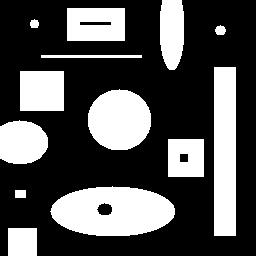
\includegraphics[width=.32\linewidth]{B.jpg}}
 \hfill
 \subfloat[Dilation.]{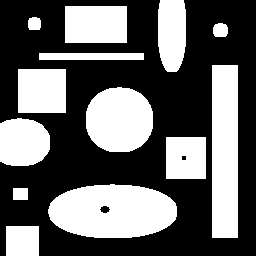
\includegraphics[width=.32\linewidth]{bm_dilatation.png}}
  
  \vspace*{-5pt}
  
 \subfloat[Erosion.]{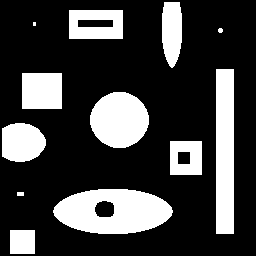
\includegraphics[width=.32\linewidth]{erosion.png}}
\hfill
 \subfloat[Opening.]{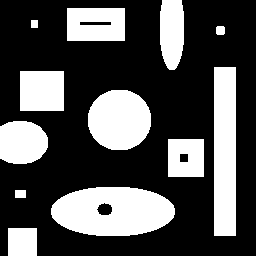
\includegraphics[width=.32\linewidth]{open.png}}
 \hfill
 \subfloat[Closing.]{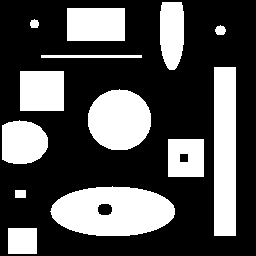
\includegraphics[width=.32\linewidth]{close.png}}%
 \vspace*{-8pt}%
 \label{python:bw_mm:basics}%
\end{figure}


\subsection{Morphological reconstruction}
The algorithm of morphological reconstruction is coded like this in python:

\begin{python}
def reconstruct(image, mask):
    # should be binary images
    M = np.minimum(mask, image);
    
    area = ndimage.measurements.sum(M);
    s=0
    
    se = np.array([[0, 1, 0], [1, 1, 1], [0, 1, 0]]);
    while (area != s):
        s = area;
        M = np.minimum(image, ndimage.morphology.binary_dilation(M, structure=se));
        area = ndimage.measurements.sum(M);
        
    return M
\end{python}

The Fig. \ref{python:bw_mm:reconstruction} illustrates the morphological recontruction.
\begin{python}
A=imageio.imread('A.jpg');
A = A > 100;
M=imageio.imread('M.jpg');
M = M > 100;
# reconstruction de A par M
AM=reconstruct(A, M);

# display results
plt.subplot(1, 3, 1);
plt.imshow(A);
plt.subplot(1, 3, 2);
plt.imshow(M);
plt.subplot(1, 3, 3);
plt.imshow(AM);
plt.show();
\end{python}
\vspace*{-10pt}
\begin{figure}[htbp]
 \centering\caption{Morphological reconstruction.}%
 \subfloat[Image $A$.]{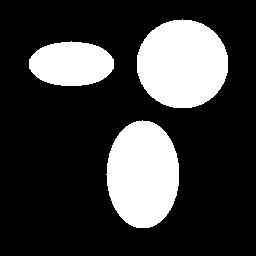
\includegraphics[width=.32\linewidth]{A.jpg}}\hfill
 \subfloat[Image $M$.]{
\includegraphics[width=.32\linewidth]{M.jpg}}\hfill
 \subfloat[\pinline{AM=reconstruct(A, M);}.]{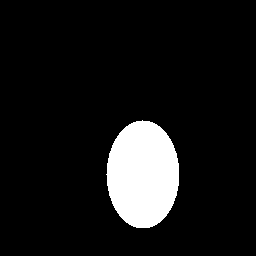
\includegraphics[width=.32\linewidth]{reconstruct.png}}%
 \label{python:bw_mm:reconstruction}\vspace*{-8pt}%
\end{figure}

\vspace*{-10pt}

\subsection{Operators by reconstruction}
\subsubsection{Remove objects touching the borders}
The Fig. \ref{python:bw_mm:borders} illustrates the suppression of objects touching the borders of the image. If $\mathcal{B}$ represents the border of the image (create an array of the same size as the image, with zeros everywhere and ones at the sides), then this operation is defined by:
\[ \textrm{killBorders}(I) = I\setminus \rho_I(\mathcal{B})\]
\vspace*{-10pt}%
\begin{figure}[htbp]
	\centering\caption{Suppress border objects.}%
	\subfloat[Original image.]{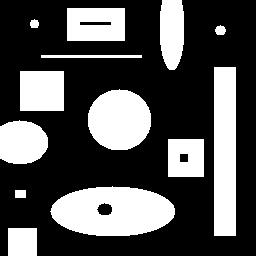
\includegraphics[width=.4\linewidth]{B.jpg}}\hfill
	\subfloat[Objects removed.]{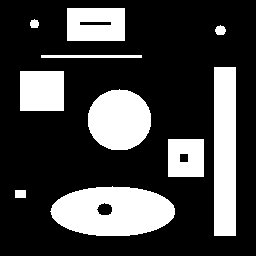
\includegraphics[width=.4\linewidth]{borders.png}}%
	\label{python:bw_mm:borders}%
	\vspace*{-8pt}%
\end{figure}

\begin{python}
def killBorders(A):
    # remove cells touching the borders of the image
    m, n = A.shape
    M = np.zeros((m,n));
    M[0,:] = 1;
    M[m-1,:] = 1;
    M[:,0] = 1;
    M[:,n-1] = 1;
    M = reconstruct(A, M);
    return A-M
\end{python}


\subsubsection{Remove small objects}
This is illustrated in Fig. \ref{python:bw_mm:small}. It consists in an erosion followed by a reconstruction. The structuring element used in the erosion defines the objects considered as ``small''.
\[\textrm{killSmall}(I)=\rho_I(\varepsilon(I)) \]
\begin{python}
def killSmall(A, n):
    # destroy small objects (size smaller than n)
    se = np.ones((n, n));
    M = ndimage.morphology.binary_erosion(A, structure=se);
    return reconstruct(A, M);
\end{python}

\vspace*{-8pt}

\begin{figure}[htbp]
 \centering\caption{Small objects removal.}%
 \subfloat[Original image.]{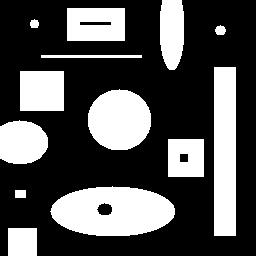
\includegraphics[width=.4\linewidth]{B.jpg}}
 \hfill
 \subfloat[Small objects are removed.]{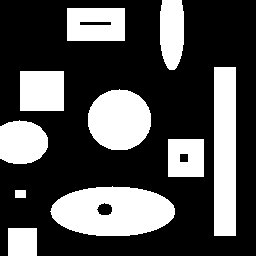
\includegraphics[width=.4\linewidth]{small.png}}%
 \label{python:bw_mm:small}\vspace*{-8pt}%
\end{figure}

\vspace*{-8pt}

\subsubsection{Close holes in objects}
This is illustrated in Fig. \ref{python:bw_mm:holes}. The operation is given by the following equation, with $\mathcal{B}$ the border of image $I$, and $X^C$ denoting the complementary of set $X$:
\[ \textrm{removeHoles(I)} = \{ \rho_{I^C}(\mathcal{B})\}^C\]
\begin{python}
def closeHoles(A):
	 # close holes in objects
    Ac = ~A;
    m,n = A.shape;
    M = np.zeros((m,n));
    M[0,:] = 1;
    M[m-1,:] = 1;
    M[:,0] = 1;
    M[:,n-1] = 1;
    M = reconstruct(Ac, M);
    return ~M
\end{python}

\vspace*{-10pt}

\begin{figure}[htbp]
 \centering\caption{Hole filling.}%
 \subfloat[Original image.]{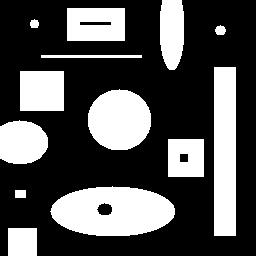
\includegraphics[width=.35\linewidth]{B.jpg}}
 \hspace*{15mm}
 \subfloat[Holes in objects are closed.]{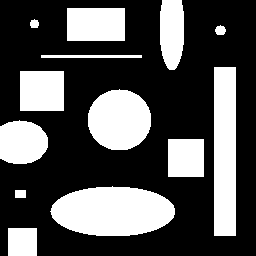
\includegraphics[width=.35\linewidth]{holes.png}}%
 \label{python:bw_mm:holes}\vspace*{-8pt}%
\end{figure}

\vspace*{-12pt}

\subsection{Application}
\textls[-10]{The application shown in Fig.~\ref{python:bw_mm:cells} presents the segmentation of blood cells after removing small cells, closing holes and removing the cells touching the borders of the image.}

\begin{python}
cells = imageio.imread('cells.jpg')<98;
imageio.imwrite('cellsbw.png', cells);
B = closeHoles(cells);
B = killBorders(B);
B = killSmall(B, 5);
plt.subplot(1,2,1);
plt.imshow(cells);
plt.subplot(1,2,2);
plt.imshow(B);
plt.title('clean image')
plt.show()
imageio.imwrite('clean.png', B);
\end{python}

\vspace*{-8pt}%

\begin{figure}[htbp]
 \centering\caption{Segmentation of the cells.}%
 \subfloat[Original image.]{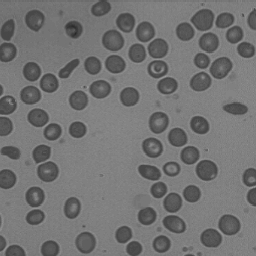
\includegraphics[width=.32\linewidth]{cells.jpg}}
 \hfill
 \subfloat[Binarization.]{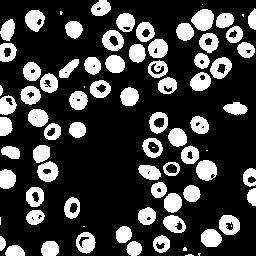
\includegraphics[width=.32\linewidth]{cellsbw.png}}
 \hfill
 \subfloat[Final segmentation of the cells.]{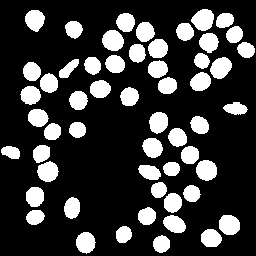
\includegraphics[width=.32\linewidth]{clean.png}}%
 \label{python:bw_mm:cells}\vspace*{-8pt}%
\end{figure}
